
\documentclass[a4paper,10pt]{article}

\usepackage[utf8]{inputenc}
\usepackage[T1]{fontenc}

\usepackage[english]{babel}

\usepackage{amsmath,amsfonts,amssymb}

\usepackage{array}

\usepackage{hyperref}

% \usepackage{float}

\usepackage{graphicx}

\usepackage{polytechnique}

  \title{AXA Data Challenge}
  \subtitle{Final Report}

  \author{Édouard MEHLMAN\\
        Raphaël OLIVIER\\
        Étienne HOUZÉ}

  \date{December 2016}

\begin{document}

  \maketitle

\begin{abstract}
  The AXA Data Challenge 2016 consisted in predicting incoming calls associated with several customer services based on a 3 Gigabits training data of recorded calls from 2011 to 2013. The main challenges for this project were the size of the training data, which required heavy preprocessing, and  the implementation of a specific loss function, the linEx function, to evaluate the performance of the prediction. The final regression was done using a tweaked version of the {\tt scikit-learn} decision tree.
\end{abstract}
\begin{center}
\rule{5cm}{0.4pt}
\end{center}

For clarity's sake, we have chosen to make an explicit separation between the preprocessing and the regression tasks. This distinction is apparent in our source code as well, each component being computed in a separate class.

\part{Preprocessing}

  A first look into the training data file showed us that, while some features needed to be created, others were useless or formatted in a way which made direct application of regression models impossible.

  It therefore appeared that it was necessary to go through various preprocessing operations before fitting the data into a regression model. This was achieved by the preprocessing class, which handles the following tasks:

    \subsection{Grouping data}

    We first noticed that some entries in the training data set were given the same tuple (DATE,ASS\_ASSIGNEMENT), which meant they corresponded to different teams from the same service. So we grouped them summing the number of calls.

    \subsection{Creating time features}

    In the orginal data, date and time features are provided as strings, which is particularily unsuitable for regression. Hence, we chose to convert them into a standardized format, which was defined, as suggested by the assignment:
      \begin{itemize}
        \item Time spent since epoch, in seconds (EPOCH)
        \item Time ellasped since start of the day, in seconds (START\_OF\_DAY)
        \item Month (MONTH)
        \item Week day (WEEKDAY)
        \item Holiday (HOLIDAY)
        \item Day off (DAY\_OFF)
        \item Week-end (WEEK\_END)
        \item Night/day (DAY\_NIGHT)
      \end{itemize}

    For the holiday and day off features, it was necessary to call a subsidiary function, isInHolday, which tested if the date was in a holiday. We provided this function a calendar, in the format of a .csv file, containing all holidays and days off in France for the years 2011-2013.

    \subsection{Handling categorical features}

    Since categorical features are not supported by regression models in {\tt scikit-learn}, we needed to format them appropriately. We ‘dummy coded’ all the categorical features (ASS\_ASSIGNMENT, WEEKDAY, HOLIDAY, DAY\_OFF), meaning, we created a new feature for every existing category, with its value in $\{0,1\}$. For instance, we changed the following lines
    \begin{center}
    {\footnotesize
      \begin{tabular}{|c|c|c|}
        \hline
        WEEKDAY \\
        \hline
        Lundi \\
        \hline
        Mardi \\
        \hline
      \end{tabular}}
    \end{center}
    into :
    \begin{center}
      {\footnotesize
        \begin{tabular}{|c|c|c|c|c|c|c|}
          \hline
          WEEKDAY\_1 & WEEKDAY\_2 & WEEKDAY\_3 & WEEKDAY\_4 & WEEKDAY\_5 & WEEKDAY\_6 & WEEKDAY\_7 \\
          \hline
          1 & 0 & 0 & 0 & 0 & 0 & 0 \\
          \hline
          0 & 1 & 0 & 0 & 0 & 0 & 0 \\
          \hline
        \end{tabular}
      }
    \end{center}

    \subsection{Normalization}

    After formatting date and time features, it was possible to normalize them, using the scaler object available in {\tt scikit-learn}. We did normalise EPOCH and START\_OF\_DAY, as it is a good practice in general when doing machine learning. However, it is not essential when using regression algorithm based on trees. This is why we didn’t normalise the others features in the dataset.

    \subsection{Handling missing values}

    We observed that there were some missing entries in our training data. Though we didn’t have the time to observe the impact of filling these missing values, we implemented a function to locate them, adding nan entries where needed, as well as function for filling these entries.

    \subsection{Selection}

    Since only 26 assignments are present in the submission data, we chose only to retain those assignments. In the end, we only used the fields (DATE,ASS\_ASSIGNEMENT,CSPL\_RECEIVED\_CALLS) from the original training data, to obtain a preprocessed version ready for regression.

\newpage
\part{Regression}

In this part, we discuss the heart of our program : the different regression models we used, and how well they fit the data.

  \subsection{Explanation of the regression class}

  We create a {\tt Regression} class for our purpose, which holds two dataframes, containing respectively the preprocessed training data and the preprocessed submission data. The {\tt Regression} class should be updated with a regressor from {\tt scikit-learn}, or any other regressor with the fit and predict functions. We can test our model with cross validation using {\tt testOnTrainData} function, that fits the regressor on one part of our training data to predict the other, and prints the resulting linEx error. After finding the proper parameters for our model, we can perform regression on the whole training data to predict the submission data and export the result with the {\tt exportResult} function. We actually created two subclasses inheriting {\tt Regression}. Indeed, we wanted to compare the performance of a single regression for the multiple assignments {\tt MultipleRegression}, against many individual regression for each assignement {\tt IndividualRegression}.

  \subsection{Building a tree using the linEx Criterion}

  The first regression model we tried to use was a decision tree. Such trees are already implemented in {\tt scikit-learn}, with ready-to-use options and parameters to fiddle with. Figure \ref{treePerf} illustrates the performance of this learner depending on its depth.

  For instance, one option lets us decide which criterion shall be used to split the data during the construction of the tree. Figure \ref{splitting} shows how the algorithm proceeds to decide where to split the feature : for each possible cut, using a specifif loss function, the splitter of the tree computes a loss both for the right and the left part of the data, to select the cut minimizing the total loss.

  \begin{figure}[h]
    \begin{minipage}{0.48\textwidth}
      \centering
      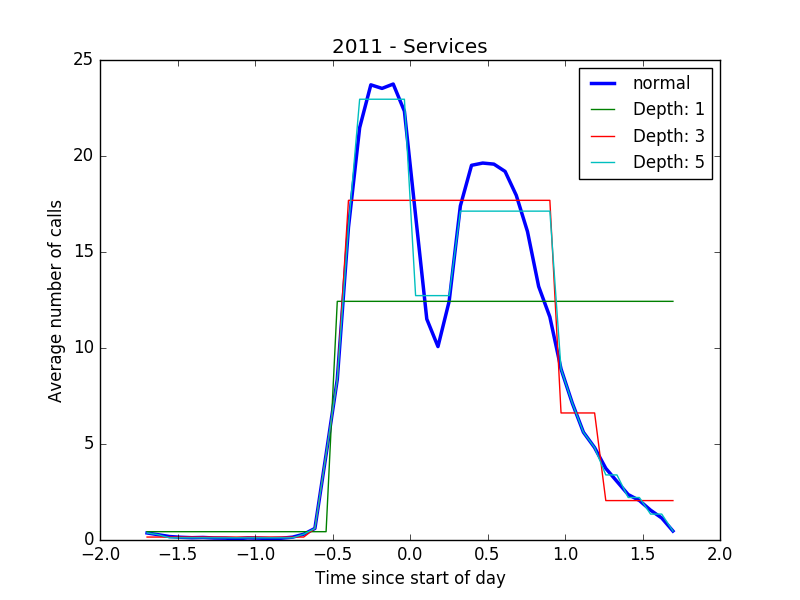
\includegraphics[width=\textwidth]{graphics/1-TreeRegression.png}
      \caption{Performance of several trees with regards to their depth}
      \label{treePerf}
    \end{minipage}
    \hfill
    \begin{minipage}{0.48\textwidth}
      \centering
      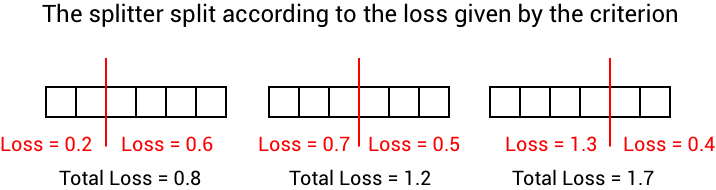
\includegraphics[width=\textwidth]{graphics/splitterpng.png}
      \caption{Visualisation of different splits}
      \label{splitting}
    \end{minipage}
  \end{figure}
  By default, the available criteria in {\tt scikit-learn} are Mean Square Estimator and Mean Absolute Estimator, each corresponding a specific loss function. However, in this assignment, the loss function to optimize is known as linEx, and is defined by :
  \begin{equation}
    \text{linEx}(y,\hat{y}) = \exp \left( \alpha (y-\hat{y})\right) - \alpha (y-\hat{y}) -1
  \end{equation}
  where $y$ is the value of a given data sample $x$, and $\hat{y}$ is its predicted value.

  Optimizing this function will optimize the quality of our prediction as computed by the linEx error. Therefore, it seemed interesting to us to implement this criterion in {\tt scikit-learn}. This trick required to fork the {\tt scikit-learn} repository to modify the source files
    \footnote{\label{note_git}The forked repository is available here : \url{https://github.com/Edouard360/scikit-learn/}}
  , written in a {\tt C++}-based language called cython in order to add an "lineEx" criterion option for the decision tree regressor.


  However, the computation of that loss for big chunks of our data required a precision up to 60 digits, which is not achievable by using {\tt double} (their precision is limited by their 64bit size). Therefore, we chose to keep the MSE loss function to split the tree. Nonetheless, we computed the node and leaf values of our tree with respect to the optimization of our loss function, and this compromise still gave us acceptable results. Figure \ref{tree_example} shows an example of a tree built using this methodology, as displayed with the {\tt export\_graphviz} function.
  \begin{figure}
    \centering
    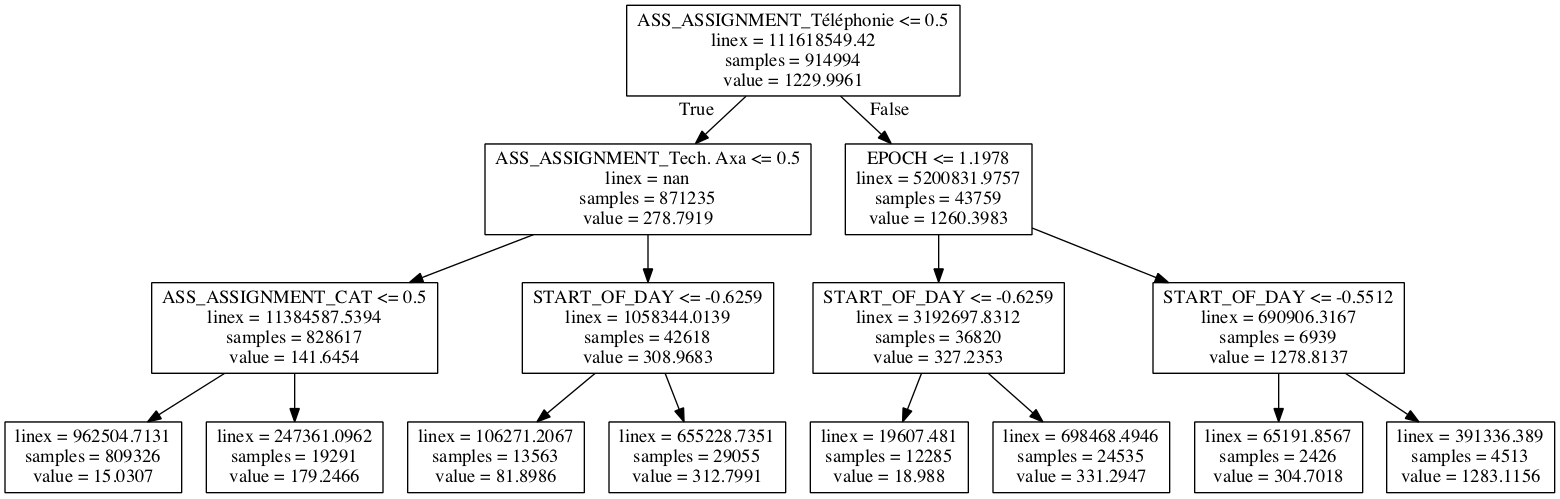
\includegraphics[width=0.8\textwidth]{graphics/tree.png}
    \caption{An example of tree built with the linEx criterion}
      \label{tree_example}
  \end{figure}

  \subsection{Use of decision trees}

  We then used decision trees in two different regression methods : \emph{bagging} and \emph{random forest}.

  The first algorithm of this type we tried was \emph{random forest}. In this learner, several decision trees are built over several random samples of data and a random sample of the original features. For every test data point, its predicted value is then the mean of the values returned by each tree. We see in figure \ref{forest} that these learners can perform significantly better than a single tree, if properly parametrized.

  \begin{figure}
    \begin{minipage}{0.48\linewidth}
      \centering
      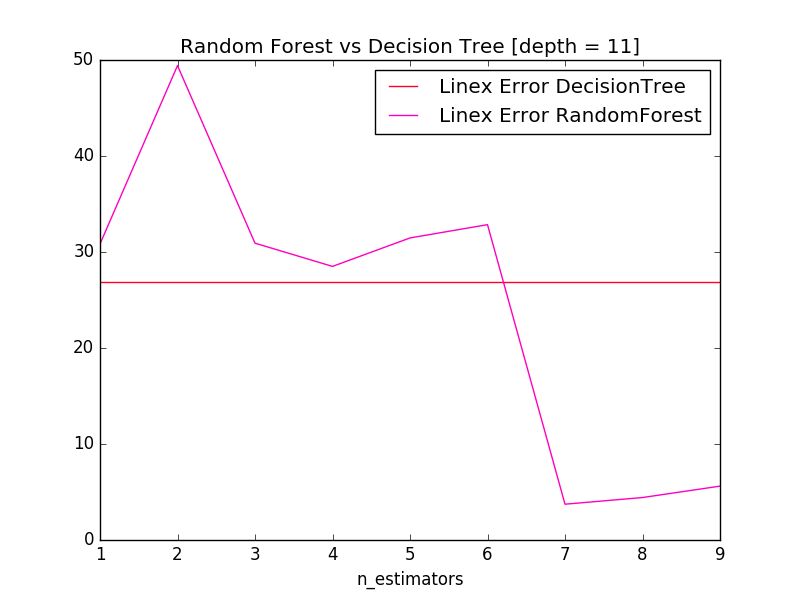
\includegraphics[width=\textwidth]{graphics/forest.png}
      \caption{Performance of random forest for various sizes}
      \label{forest}
    \end{minipage}
    \hfill
    \begin{minipage}{0.48\linewidth}
      \centering
      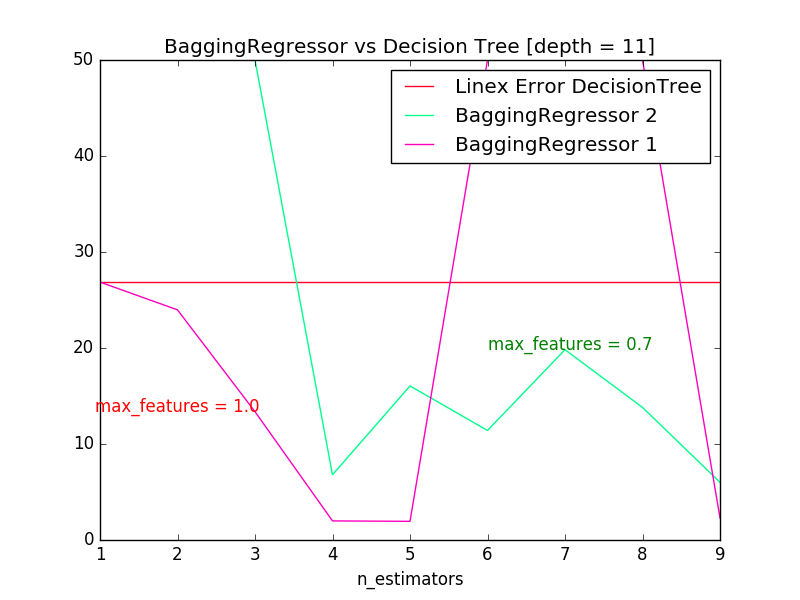
\includegraphics[width=\textwidth]{graphics/Bagging.png}
      \caption{Performance of Bagging algorithms based on decision trees}
      \label{bagging}
    \end{minipage}
  \end{figure}

  The {\tt BaggingRegressor} from {\tt scikit-learn} does essentially the same, though it can be set with any given base regressor - not necessarily a tree as it is the case for a forest. This learner is not very stable for a small number of estimators as shown in Figure \ref{bagging}, but can score particularly well if parameters are well chosen.

  \subsection{Tracks for improvement}

  We observed that our data could be predicted using time series analysis. Its statistical features such as mean, variance and covariance do not evolve much throughout time. Such properties could be explored in a yet completely different regression model, but due to a lack of time, we chose to focus on the work thereabove explained.

  \begin{figure}
    \centering
    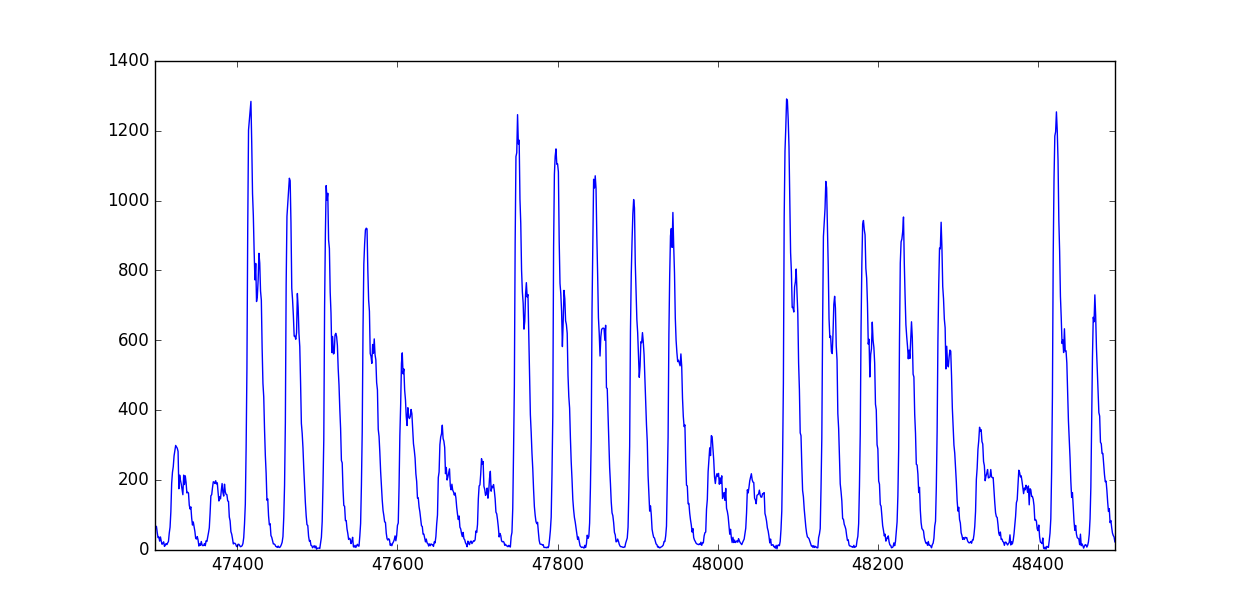
\includegraphics[width=0.8\textwidth]{graphics/3-Time_series.png}
    \caption{Evolution of the data with regards to the time. The y-axis represents the number of calls plotted with regards to the time.}
    \label{time_series}
  \end{figure}

\part{Conclusion}

  For our team, the best results were obtained by performing random forest regression after tweaking a decision tree criterion provided by {\tt scikit-learn} to take into account the linEx loss function. We had to make compromise in its implementation, and probably better results would have been achieved with a tree splitted according to the Linex loss function.

%   \subsection*{The Linex loss function}
%
%
% \vspace{1 cm}
% \label{norms}
% We have the loss function defined by:
%     $$loss = \sum_{i=1}^{n} (e^{\alpha (y_i-y_{pred})} - \alpha  (y_i-y_{pred}) - 1)$$
%
%
% Its \textbf{derivative} defined by:
%     $$ \frac{\partial loss}{\partial y_{pred}} = \sum_{i=1}^{n} (-\alpha e^{\alpha (y_i-y_{pred})} + \alpha)$$
%     $$ \frac{\partial loss}{\partial y_{pred}} = -\alpha e^{-\alpha y_{pred}} \sum_{i=1}^{n} ( e^{\alpha y_i} ) + n\alpha$$
%
%
%
%
% Looking for the \textbf{minimum}, we have:
%     $$ \frac{\partial loss}{\partial y_{pred}} = 0 \implies
%     e^{\alpha y_{pred}} = \frac{\sum_{i=1}^{n} (e^{\alpha y_i})}{n}$$
%     $$ y_{pred} = \frac{1}{\alpha} \log(\frac{\sum_{i=1}^{n} (e^{\alpha y_i})}{n})$$
%
%
%
%
% Replacing this value in the loss, we obtained the \textbf{minimum loss}, ie. the minimum impurity of the data.
%     $$loss = n\log(\frac{\sum_{i=1}^{n} (e^{\alpha y_i})}{n}) - \sum_{i=1}^{n} \alpha y_i$$
%
%
%
%
% And we can verify, using the Jensen inequality that:
%     $$loss >= 0$$



\end{document}
